%%%%%%%%%%%%%%%%%%%%%%%%%%%%%%%%%%%%%%%%%%%%%%%%%%%%%%%%%%%%%%%%%%%%%%%%%%%%%%%%%%%%%%%%%%%%%%%%%%%%%%
%
%   Filename    : chapter_3.tex 
%
%   Description : This file will contain your Research Methodology.
%                 
%%%%%%%%%%%%%%%%%%%%%%%%%%%%%%%%%%%%%%%%%%%%%%%%%%%%%%%%%%%%%%%%%%%%%%%%%%%%%%%%%%%%%%%%%%%%%%%%%%%%%%

\chapter{Theoretical Framework}
This chapter contains theories and concepts that are related to the research.

\section{Symphonies}
\subsection{Basic Structure of a Symphony}
The Classical and Romantic symphony is mainly written in four movements, namely the fast tempo or sonata allegro form, the slow tempo, the medium/fast tempo or minuet, and the fast tempo again. The sonata form makes up the main form of Classical and Romantic symphonies. It is composed of two contrasting themes, the aggressive and the passive and is further divided into several sections, namely the introduction, exposition, development, recapitulation, and coda. The introduction section is purely optional and is slow and solemn in nature. The exposition section is where the themes of the symphony are “exposed” or presented for the first time and will consequently be repeated all throughout. The development section is where the themes are altered and manipulated. The recapitulation section is where the themes return to their original forms from before they were altered. The code section finally represents the end of the movement and this is where the original tone from the exposition section is repeated or recapped to form the ending for the movement (Heikkinen, 2017 \& BBC, 2014).

\subsection{Music Features}

A feature is a characteristic used to distinguish one entity from another and in a sense defines its uniqueness. Music features, therefore, are what makes music similar to or different from one another. By comparing the values  for each music feature and by examining if a feature is present at all or not, comparison of music by mathematical means is very possible (Huron, 2001).

Today, music information retrieval (MIR) has become an important area of research especially because of the ever expanding database for music through the years. The features extracted from music can be used in many areas of MIR research. It can be said that when two songs share closer values for each music feature, then they are more similar than with others (Corrêa \& Rodrigues, 2016).

\subsubsection{MFCC}

MFCC, also known as Mel-Frequency Cepstral Coefficients, is the most commonly used feature in speech analysis and since speech analysis and music research are closely interrelated as pointed out by Loughran, Walker, O’Neill, \& O’Farrell (2008), then MFCC will likely be the most commonly used feature in music feature extraction.

According to Lutter (2014), MFCC is based mainly from experiments on human misconceptions of words such as when a person misunderstands what another person says. This feature extraction method was first developed by Bridle and Brown in 1974 and was further developed by Mermelstein (1976).  The MFCC feature extraction method involves mimicking some parts of the human speech production and speech perception. This feature extraction involves five steps, namely the fourier transform, the mel-frequency spectrum, the logarithm, cepstral coefficients, and the derivatives. The first step, fourier transform makes use of the formula $C_r,_k=| \frac{1}{N}\sum_{j=0}^{N-1} fj exp [-i 2 \pi \frac{jk}{N}]|$, where $k=0,1,...,(\frac{N}{2})-1$ and N is the number of samples within a speech or time frame.

The mel-frequency spectrum closely mimics the sensation of the human ear’s auditory system and the process involves filtering the spectrum with different band-pass filters, devices that pass frequencies within a certain range and reject all others, and the power for each band-pass filter is computed accordingly (Agarwal, 2017). The computation makes use of the formula $C_T,_j=\sum_{k=0}^{\frac{N}{2}-1} d_j,_k C_T,_k $, where $j=0,1,...,N_d$ and d is the amplitude of the band-pass filters at index j and frequency k, to produce the corresponding filter bank for the spectrum.

The third step, logarithm involves mimicking the perception of loudness by the human ear and is represented by the formula $C_T,_j= log(C_T,_j)$  where $ j=0,1,...,N_d$.

In cepstral coefficients, the main goal here is to remove the speaker or the music dependent characteristics. The computation of cepstral coefficients results in the inverse of the fourier transform of the estimated spectrum of the signal and is represented by the formula $C_T,_j=\sum_{j=1}^{N_d} C_T,_j cos[\frac{k(2j-1)\pi}2N_d]$ where $k=0,1,...,N_m,_c<N_d$ and $N_m,_c$ is the chosen cepstral coefficient for further processing.

Lastly, the derivative represents the dynamic nature of speech or the music.

\section{Preprocessing}
\subsection{Data Collection}

In gathering data, a careful lookup for patent or copyright issues must strictly be observed. Symphonies are musical pieces that were generally composed a long time ago and as such copyright on the actual symphonies are nonexistent. The only copyright issues to be possibly encountered here would be the source of the recreated symphony. For example, when the symphony is uploaded by a certain person in Youtube then the standard youtube license or the creative commons would apply (Brown,  2017).

\subsection{Preparation of Dataset}

In Azcarraga \& Flores (2016)’s research regarding visualization and comparison of symphonies through SOM, the preparation of dataset was done by first cutting the symphony into multiple 1 second music segments with an overlapping interval of 0.5 second to provide a smoother transition of the segments when represented later visually in addition to taking consideration of sections or notes that have been abruptly cut during the splitting process. In this way, after the feature is extracted and trained in the SOM, the multiple music segments will make up different musical trajectories which makes up the map visualization.

\subsection{Feature Extraction}

Feature extraction is the means of extracting relevant and effective data to train machine learning algorithms. Not all features, however, may be useful and others may be irrelevant individually but can be useful when combined with other features. The input data or “raw” data often need to be converted into a set of useful features through preprocessing transformations such as, standardization, normalization, signal enhancement, nonlinear expansion, et al. The resulting data may also be pruned of excess features in order to achieve improved algorithm speed and or predictive accuracy (Guyon \& Elisseeff, 2006).


Feature extraction for music can be done using JAudio, a Java project/program developed by McEnnis, McKay, Fujinaga, \& Depalle (2005). JAudio is a feature extraction system that provides a user friendly GUI and a command line interface to suit user needs for selecting their desired features to be extracted for the audio. The system accepts audio files as input and outputs XML or ARFF files. This output file contains the values for each feature of the audio file selected by the user.

\subsection{Feature Selection}

Gupta (2017) defines decision tree as a binary tree that branches down from the root. The term tree-walking is used to continuously make decisions on every level of the tree starting from the root node until the leaf nodes are reached or a satisfactory answer is found. In this way, it can be derived that the nodes found at the top of the tree are more important than its child nodes and all others beneath them. Decision trees are useful for inferring what features of a dataset can greatly or weakly influence its outcome (Mitchell, 1997).

Feature selection is the automatic selection of attributes in the dataset that are most relevant to a specific predictive model. Feature selection helps in reducing the number of data attributes being used while still retaining a good or accurate predictive model. Aside from reducing the number of features or data attributes, it can also help in removing unwanted attributes that may decrease the accuracy of the predictive model (Brownlee, 2014).

Grabczewski \& Jankowski (2005) explains that decision tree algorithms are best used for feature selection because of the inherent characteristic of decision trees that allows them to separate the different features and showcase the more important features since it will appear on top of the decision tree.
	
	Some simple but successfully tested algorithms for feature selection would include Pearson’s correlation coefficient and Fisher-like criterion. Pearson’s correlation coefficient or Pearson’s R is widely used in the computation of statistics and this involves detecting linear correlation, which is the representation of how close the data points are in making a straight line in a graph, just as shown in Figure 3.1. In feature selection, Pearson’s correlation coefficient can produce poor results when presented with nonlinear data structures; however, it is still a reliable algorithm for feature selection because of its simplicity and optimal results for most cases.

\begin{figure}[h]
\caption{Figure 3.1)}
\centering
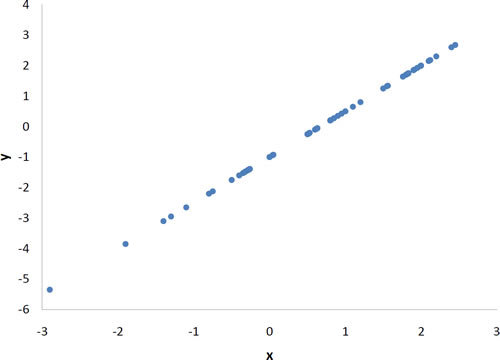
\includegraphics{pearson}
\end{figure}

Fisher-like criterion makes use of the formula $\frac{m_0-m_1}{s_0-s_1}$, wherein m is the mean value of the feature for the$i$-th element and $s$ is the corresponding standard deviation. This algorithm can only be used, however, when dealing with binary classifications.

Feature selection, in general however, can be classified into three categories, namely the filter methods, wrapper methods, and the embedded methods. Filter method involves labelling each feature with a statistical measure and by comparing these measures, the more important features can be selected. Wrapper method involves grouping different combinations of features together to see which combinations work best. Embedded methods involve learning which features best contribute to the accuracy of the model while the model is simultaneously being created. Some more examples of feature selection algorithms would include best-first search, hill-climbing algorithm, and the usage of heuristics. The first two fall under the wrapper methods wherein different combinations are used until the top n features are found. The last one falls under the filter method wherein a heuristic score is given to each feature using a statistical measure such as Euclidean distance for example, and the features with the high scores will be the ones selected.For this reason, The proponents will use Decision trees in order to find which features can be ignored during SOM construction. As a result of reducing the number of features for training the SOM will have a decrease in the accuracy of the generated map, however, using a lower number of features allows faster training of the SOM. The resulting  decision tree will be used to determine unnecessary nodes and trim down the number of features to the 20 most influential features where 20 is an arbitrary number chosen by the proponents.

\section{Machine Learning}

Machine learning as defined by Ng (2017) in his online course for machine learning in Stanford University is the science behind computers acting on a certain stimulus without being explicitly programmed to do so. Some examples of impact led by machine learning would be self-driving cars and web search suggestions from Google. Machine learning is also widely used in many different fields of research such as in artificial intelligence, data mining, natural language processing, image recognition, and expert systems (McCria, 2014). In machine learning, the concept of training the system to perform a unique task given a certain amount of data received has two main underlying categories, unsupervised learning and supervised learning.

\subsection{Unsupervised Learning}

Brownlee (2016) defines unsupervised learning as having only one input and having no corresponding output variable. Unsupervised learning is analysing the structure and distribution of the data in order for system to learn. It is called unsupervised because unlike supervised  which requires the supervision of a person to correct learned data, unsupervised learning leaves the algorithm on its own to learn from the data. Unsupervised learning can be further classified into two groups of algorithms, namely the clustering and the association. Clustering is used for discovering the groupings of data through clusters and association is used for discovering rules that describe the provided data.

\subsubsection{SOM}
Germano (1999) defines SOM as a data visualization technique developed by Professor Teuvo Kohonen which reduces the dimension of data through the use of self-organizing neural networks. As SOM reduces the dimension of data, it also groups similar data items together; therefore, it not only reduces the dimension of data but also groups similar ones together. Figure 3.2 shows a basic example of a SOM. Note in this example that the data represented by colors are grouped according to their similarity (eg. yellow is near orange, dark teal is between blue and green).

\begin{figure}[h]
\caption{Figure 3.2)}
\centering

\includegraphics{som}
\end{figure}

Bullinaria (2004) defines a class under supervised learning called competitive learning. Here, neurons compete among themselves in a winner-takes-it-all scenario wherein only one neuron wins and is activated at any one time. Implementation of this competition is done through the use of lateral inhibition connections, which are structures of a network in which neurons inhibit their neighbors (Kropotov, 2009). When neurons are forced to organize themselves through this scenario, then the result would be a map that is self-organized, thus a SOM.

\subsubsection{K-Means Clustering Algorithm}

K-means clustering algorithm is a type of unsupervised learning algorithm wherein a set of unlabeled data will be grouped together and these groups are defined as the k variable. The algorithm will assign the different data points to their respective k-groups based on the selected features. Data points will then end up being clustered based on their feature similarities. The algorithm has two main iterative steps, , the data assignment step and the centroid update step, that repeats until either data points change clusters, the sum of the distances is minimized, or some maximum number of iterations is reached. Before starting with these two steps, the centroid for each k-cluster is computed first. In data assignment, each data point is placed in their nearest centroid value computed with squared Euclidean distance. In centroid update, the centroid is recomputed by taking the mean of all the data assigned to the centroid’s cluster (Trevino, 2016; Hartigan \& Wong, 1979). 

\subsection{Supervised Learning}

Supervised learning, as defined by Brownlee (2016), is a type of machine learning wherein an input variable and an output variable is defined and an algorithm is used to map the input to the output variable. The goal of this type of learning is to map the input variables to their respective output variables by approximation so that when a new input variable is presented, an output can be predicted by the system. The main difference of supervised learning over unsupervised is that there is no third party that supervises and corrects the training of data in unsupervised but in supervised, intervention of the supervisor is necessary in order to achieve an acceptable level of performance by the system. Supervised learning can be further divided into two groups, namely regression and classification. Regression is used when the output is a real value, for example, weight, height, or age. Classification is used when the output is a category or group, for example, colors, sizes.

\section{Visualization}
\subsection{Single Image}

Just as done in Azcarraga \& Flores (2016) research work, visualization for the result of the SOM can be done in a single image. The BMU or best matching unit, which will be explained further in section 3.5.1, represents the music trajectory of a certain 1 second music segment from the symphony. This sequence of BMUs make up the visual image representation of a certain symphony. A color coding scheme was also used to denote the time sequence of a certain music trajectory in the image, blue representing the start and going to red as the music progresses as shown in Figure 3.3.

\begin{figure}[h]
\caption{Figure 3.3)}
\centering
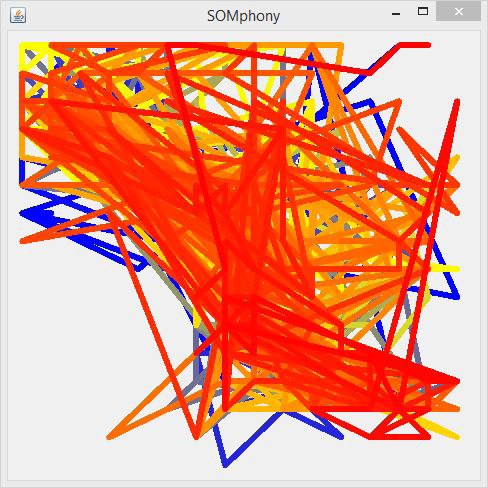
\includegraphics[width=0.5\textwidth]{somphony_sample}
\end{figure}

\subsection{Video}
Aside from representing the result of the SOM in a single image, it can also be represented in a video or multiple images. Video can be produced for the results of this research by collating  each 1 second segment result in order to show the progression of the musical trajectory grow from the start of the symphony to the end. This allows clearer visualization of the data to have more accurate analysis. Using this kind of visualization also greatly helps the survey user in the outcome of this research.

\subsection{3D Models}

In Azcarraga, Caronongan,  Setiono, \& Manalili (2016)’s research work, they incorporated the use of a structured 3D SOM instead of the regular SOM which will result in a single image. They represented the 3D map as a 3x3x3 dimensional cube with 27 subcubes each of the same sizes. Each subcube is further divided into 9x9x9 nodes. Here, they introduced the concept of a core cube at the center and the other 26 corresponding exterior cubes surrounding it. The training phase of the cube involved a four step labelling phase which was discussed in greater detail back in chapter 2. The resulting 3D SOM was then used to identify the proximity of a certain music to a particular genre. Each genre represented one corner of the cube as shown in Figure 3.4.

\begin{figure}[h]
\caption{Figure 3.4)}
\centering
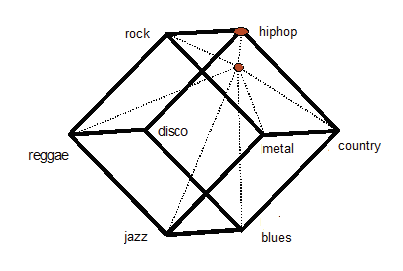
\includegraphics[width=0.5\textwidth]{cube}
\end{figure}

\section{Metrics}

There are two general types of data, qualitative and quantitative data. Qualitative data are data that cannot be measured by numbers while quantitative can be measured by numbers.

\subsection{Quantitative}

When using clustering as the method for machine learning, for example k-means clustering, there will result in k number of clusters after the algorithm is performed. Azcarraga \& Flores (2016) used k-means clustering in clustering the 1 second music segments. The best matching unit (BMU) for each 1 second music segment is first computed using Euclidean distance, which is the square root of the square of the difference between the x-axis of the first and second point added to the square of the difference between the y-axis of the first and second point, as shown in Figure 3.5.

\begin{figure}[h]
\caption{Figure 3.5)}
\centering
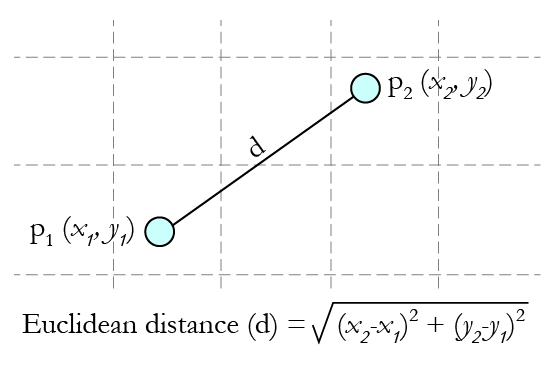
\includegraphics[width=0.5\textwidth]{euclidean}
\end{figure}

Each time a 1 second music segment has a BMU inside a cluster, the frequency count for that cluster is incremented. In this way, only the clusters that are mainly used by the music or symphony will have a high frequency count. The frequency counts are then normalized by dividing the counts of a certain composition by its total number of 1 second music segments. Once these normalized frequency counts are summarized, the resulting percentages can then be used to perform pair-wise comparisons between symphonies as shown in Appendix D.

\subsection{Qualitative}

In theory, the main purpose of conducting surveys is to generate results for a certain research work; however, surveys can also be used to validate the results of a research by comparing the results of the surveys and the results produced initially by the research work. In performing research regarding the usage of algorithms in visualizing and comparing symphonies, it would be sound to say that performing surveys that require participants to listen to two symphonies that have been calculated by the SOM to have a large degree of similarity and asking the surveyees for their opinion on the closeness of the two symphonies can help validate the research work if it really produced reliable or accurate results.

\nocite{Dubnov}
\nocite{Azcarraga2016}
\nocite{cambouropoulosEmilios}
\nocite{3dsom}
\nocite{correa}
\nocite{imogen}
\nocite{libin}
\nocite{foote}
\nocite{silla}
\nocite{mcfee}
\nocite{hepokoski}
\nocite{heikkinen}
\nocite{bbc}
\nocite{huron}
\nocite{mckay}
\nocite{mcennis}
\nocite{loughran}
\nocite{lutter}
\nocite{mermelstein}
\nocite{agarwal}
\nocite{iitg}
\nocite{ng}
\nocite{mccria}
\nocite{brownlee}
\nocite{germano}
\nocite{bullinaria}
\nocite{kropotov}
\nocite{grabczewski}
\nocite{gupta}
\nocite{brownlee1}
\nocite{trevino}
\nocite{hartigan}
\nocite{brown}
\nocite{ziv}
\nocite{ron}
\nocite{mitchell}
\nocite{guyon}
\nocite{yang}